\subsection{Kiến trúc tổng quan của hệ thống}
Hình~\ref{fig:system_architecture} mô tả luồng dữ liệu từ ảnh đầu vào và cấu hình chung đến hai nhánh tính toán và hai tầng đánh giá. Cùng một ảnh và tỷ lệ được đưa vào nhân NumPy và bộ tham chiếu Fiji/FeatureJ. Các phép xử lý cần thống nhất kiểu dữ liệu, bậc đạo hàm, đơn vị, quy ước chuẩn hóa và cách loại bỏ vùng biên trước khi đối chiếu.

\begin{figure*}[t]
\centering
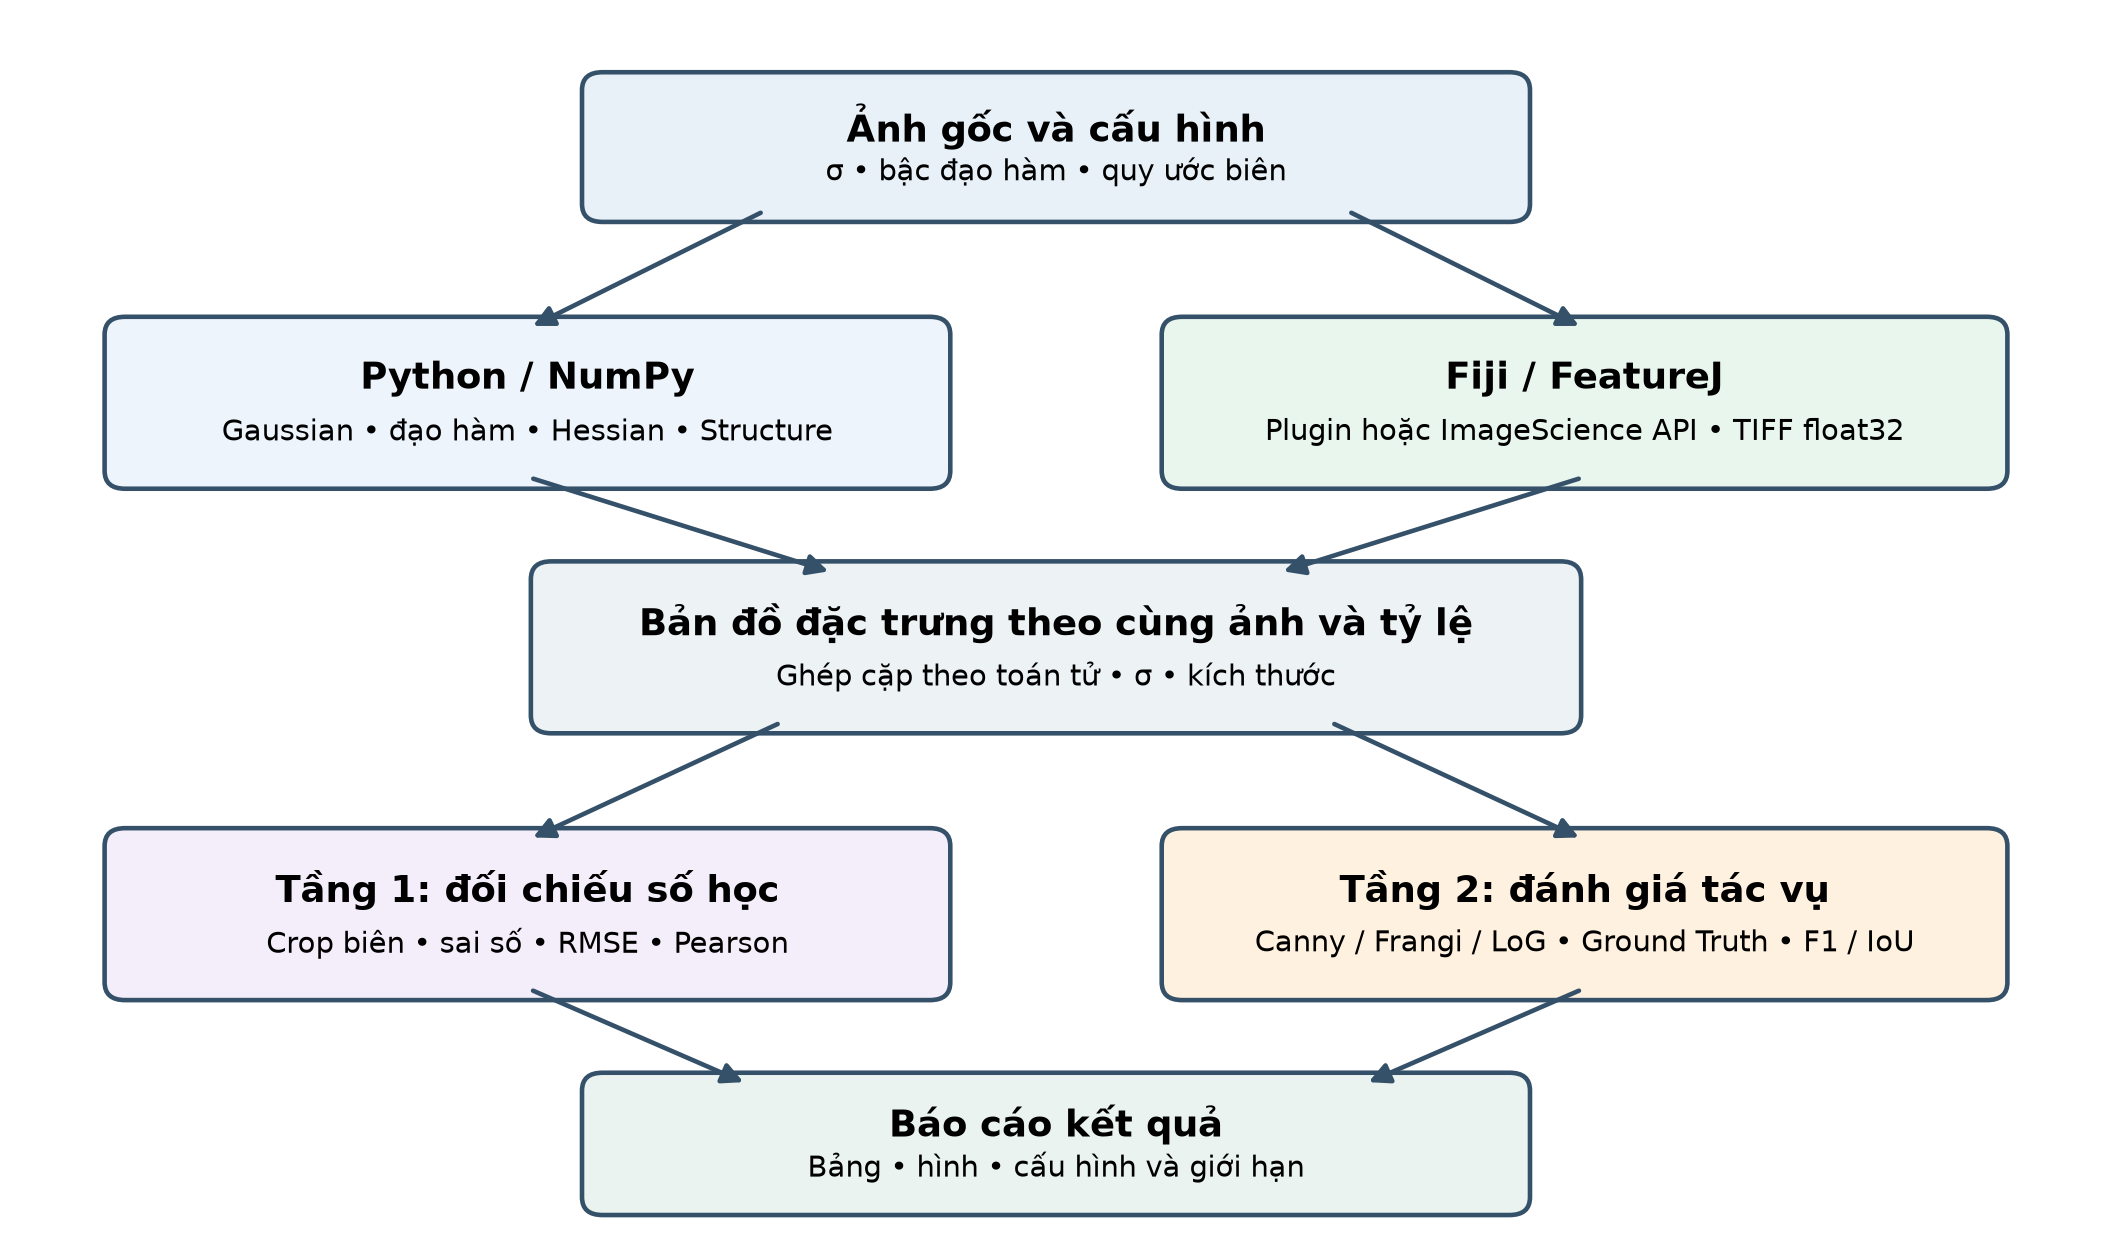
\includegraphics[width=0.94\textwidth]{figures/system_architecture.png}
\caption{Kiến trúc xử lý và đánh giá của dự án: hai nhánh tính bản đồ đặc trưng, đối chiếu số học ở Tầng 1 và đánh giá tác vụ với Ground Truth ở Tầng 2. Sơ đồ mô tả quy trình tổng quát; bộ chạy mẫu mới chỉ bao gồm ba ảnh và sáu toán tử.}
\label{fig:system_architecture}
\end{figure*}

Ở Tầng 1, các bản đồ cùng ảnh, toán tử và tỷ lệ được ghép cặp để tính sai số và Pearson trên vùng hợp lệ. Ở Tầng 2, các bản đồ đặc trưng đi qua thuật toán phát hiện tương ứng rồi so với nhãn tham chiếu; F1 và IoU phản ánh kết quả tác vụ theo giao thức đã chọn. Chẳng hạn, nhánh Fiji của phép so sánh Canny công bằng cung cấp $L_x,L_y$ rồi dùng cùng bước hậu xử lý Python; kết quả FeatureJ Edges được báo cáo riêng. Sơ đồ không hàm ý rằng phiên GUI bổ sung đã chạy lại toàn bộ benchmark của nhóm.

\subsection{Vai trò của Fiji/FeatureJ và mã nguồn Python trong báo cáo}
Fiji là môi trường xử lý ảnh dựa trên ImageJ; FeatureJ là bộ plugin cung cấp các phép trích xuất đặc trưng vi phân \cite{meijeringFeatureJ}. Trong đề tài này, Fiji/FeatureJ cung cấp một bộ cài đặt độc lập để kiểm tra nhân NumPy. Repo cung cấp nhân tính toán, dữ liệu, cấu hình, macro và bộ đánh giá. Hai thành phần cần được nối bằng cùng ảnh đầu vào và cùng quy ước tham số để phép so sánh có ý nghĩa.

Tài liệu yeucau.md của repo yêu cầu workflow Fiji, cài đặt thuật toán và đối chiếu định lượng giữa công cụ với code nhóm; không quy định từng thành viên phải tự chạy lại toàn bộ dữ liệu. Người viết báo cáo có thể tổng hợp kết quả nhóm đã tạo nếu chỉ rõ nguồn. Để bảo đảm hiểu workflow và có minh chứng thực hành, phương án trong bản báo cáo này là chạy lại một tập nhỏ, đồng thời dùng CSV của nhóm cho các bảng tổng hợp. Các kết quả nhóm có sẵn và kết quả mới phải có nhật ký riêng.

\subsection{Chuẩn bị môi trường và kiểm tra đầu vào}
\subsubsection{Fiji và plugin}
Tải Fiji từ nguồn chính thức, giải nén vào thư mục có quyền ghi, mở chương trình rồi dùng trình cập nhật để bật update site ImageScience. Sau khi cập nhật và khởi động lại, kiểm tra các lệnh FeatureJ Derivatives, Edges, Laplacian, Hessian và Structure xuất hiện. Không chỉ kiểm tra tên plugin: cần mở thử một ảnh xám và xác nhận một phép đạo hàm chạy thành công.

Ghi lại phiên bản Fiji/ImageJ, Java, FeatureJ và ImageScience trong nhật ký chạy. Các tên cửa sổ đầu ra và lựa chọn của hộp thoại có thể thay đổi theo phiên bản; công cụ Macro Recorder của ImageJ giúp kiểm tra chuỗi tùy chọn thực sự được gửi tới plugin trên máy đang dùng.

\subsubsection{Môi trường Python}
Repo sử dụng NumPy trong nhân toán học; Pillow để đọc PNG, tifffile để trao đổi TIFF float, PyYAML để đọc cấu hình, SciPy trong một số bước đánh giá và Matplotlib để vẽ. Cần tạo môi trường riêng, cài theo requirements.txt của repo, rồi ghi lại phiên bản thực tế thay vì coi danh sách phiên bản đề xuất trong README là phiên bản máy đã cài.

Mọi lệnh chạy nên bắt đầu từ thư mục gốc của repo, nơi chứa config.yaml, data và src. Kiểm tra ảnh cùng nhãn đã có trước khi chạy. Một repo chỉ có mã mà thiếu dữ liệu hoặc kho TIFF tham chiếu sẽ chưa đủ để tái lập toàn bộ bảng.

\subsection{Thí nghiệm mẫu đề xuất}
Chọn ba ảnh đại diện: bsds\_01 cho biên, drive\_01 cho cấu trúc mạch và blob\_01 cho đốm tổng hợp. Dùng $\sigma=\{1,2,4,8\}$ và giữ nguyên kích thước ảnh. Bộ chạy mẫu kèm báo cáo xuất $L,L_x,L_y,L_{xx},L_{xy},L_{yy}$ cho mỗi ảnh và tỷ lệ: tổng cộng $3\times4\times6=72$ bản đồ trên mỗi nhánh.

Tập này dùng để kiểm tra thao tác, đọc bản đồ và đo sai khác toán tử. Nó không thay thế benchmark 25 ảnh và không đủ để đưa ra kết luận tổng quát về ba bộ dò. Khi cần minh họa độ khó của dữ liệu sinh học, mở thêm blob\_05 và đối chiếu với kết quả tổng hợp trong CSV nhóm.

\subsubsection{Quy trình thao tác trên một ảnh}
\begin{enumerate}
\item Mở đúng PNG từ data/raw và ghi lại tên file. Không dùng ảnh chụp màn hình hoặc bản JPEG có nén thay cho ảnh gốc.
\item Đặt đơn vị không gian là pixel, sau đó chuyển ảnh làm việc sang 32-bit. Không thay đổi dải cường độ độc lập cho từng nhánh.
\item Chạy FeatureJ Derivatives tại cùng $\sigma$: bậc $(0,0)$ cho Gaussian, $(1,0)$ cho $L_x$, $(0,1)$ cho $L_y$, $(2,0)$ cho $L_{xx}$, $(1,1)$ cho $L_{xy}$ và $(0,2)$ cho $L_{yy}$. Với ảnh một lát, bậc theo $z$ bằng 0.
\item Lưu mỗi bản đồ bằng TIFF 32-bit. Tên file ghi rõ ảnh, toán tử và $\sigma$; không ghi đè ảnh gốc.
\item Chạy nhân Python trên cùng PNG và xuất cùng sáu toán tử. Chỉ đối chiếu các cặp đã khớp ảnh, kích thước, toán tử và tỷ lệ.
\item Loại vùng biên theo bán kính hỗ trợ kernel trước khi tính sai số. Lưu cả giá trị số và một hình ghép để đọc trực quan.
\end{enumerate}

\subsection{Phân biệt bản đồ gradient và đầu ra biên}
Trong FeatureJ Edges, tính gradient, NMS và phân ngưỡng là các lựa chọn liên quan nhưng khác nhau. Gradient chưa NMS thường tạo dải đáp ứng rộng; bản đồ sau NMS mảnh hơn; ảnh sau hysteresis là kết quả nhị phân. Nếu lấy một ảnh nhị phân so với gradient float, sai khác sẽ chủ yếu phản ánh khác tầng xử lý.

Ở nhánh BSDS dùng cho so sánh công bằng trong repo, Fiji xuất $L_x,L_y$; Python nhân $\sigma$ và đưa chúng qua cùng detect\_canny như nhánh NumPy. Các ngưỡng được chọn trên Python rồi giữ cố định khi áp cho Fiji. FeatureJ Edges có NMS nội bộ là tham chiếu riêng với ngưỡng tuyệt đối riêng; F1 của nó được báo cáo ở cột riêng \cite{xlaRepository}. Do đó, cột mang tên Fiji trong bảng fair không đồng nghĩa toàn bộ pipeline Canny được thực thi trong plugin.

\subsection{Hessian, Structure Tensor và cực tính}
Khi xuất Hessian để đối chiếu, chọn hai trị riêng lớn nhất/nhỏ nhất theo thứ tự đại số, giữ nguyên dấu. Chỉ sắp theo độ lớn khi bước Frangi yêu cầu. Đối với ảnh DRIVE có mạch tối, độ cong mạnh ngang mạch là dương theo quy ước cường độ của ảnh; dùng tiêu chí ridge sáng sẽ làm mất phần đáp ứng cần quan tâm.

Với Structure Tensor, đặt riêng tỷ lệ vi phân và tích phân theo config.yaml: $(1,3)$ và $(2,6)$. Ghi cả hai vào tên file. Không dùng nhầm $\sigma_i$ làm tỷ lệ tính gradient, vì khi đó tensor vẫn có hình dạng hợp lý nhưng không còn là cùng phép đo với nhánh Python.

\subsection{Các nguồn tham chiếu và nguồn gốc đầu ra}
Bộ 220 TIFF của Java Exporter gọi ImageScience được dùng cho Tier 1. Bộ outputs/fiji của workflow macro phục vụ minh chứng công cụ và Tier 2. Theo README hiện hành, bộ macro gồm 423 TIFF trong phạm vi macro hợp nhất và 12 TIFF edge cũ được giữ lại, tổng 435 TIFF. Vì vậy không mô tả 435 file như sản phẩm của một lần chạy mới duy nhất nếu chưa có nhật ký xác nhận \cite{xlaRepository}.

Macro hiện hành batch\_process.ijm đọc config.yaml và bỏ qua một số file đầu ra đã tồn tại. Cơ chế này hữu ích để chạy tiếp, nhưng việc nhấn Run rồi thấy kết thúc không chứng minh mọi file vừa được tính lại. Khi cần đo thời gian hoặc tạo minh chứng mới, dùng thư mục đầu ra thí nghiệm riêng và lưu danh sách file được tạo trong lần chạy đó.

\subsection{Minh chứng cần thu thập cho báo cáo và bảo vệ}
\begin{table*}[t]
\centering
\caption{Minh chứng thực hành và câu hỏi mà mỗi minh chứng trả lời}
\begin{tabularx}{\textwidth}{lXX}
\toprule
Minh chứng & Nội dung cần ghi & Ý nghĩa\\
\midrule
Cấu hình phần mềm & Phiên bản, update site, lệnh FeatureJ & Xác nhận đúng môi trường tham chiếu\\
Ảnh gốc và metadata & Tên, kích thước, kiểu dữ liệu, đơn vị pixel & Xác nhận hai nhánh dùng cùng đầu vào\\
Hộp thoại lọc & Toán tử, bậc đạo hàm, $\sigma$, lựa chọn trị riêng & Cho phép tái lập phép đo\\
TIFF float và CSV & Bản đồ số gốc, sai số sau crop, trạng thái thiếu file & Cho phép kiểm tra định lượng\\
Hình ghép & Ảnh gốc, Python, Fiji, sai khác cùng thang màu & Giúp đọc vị trí và dạng sai khác\\
Nhật ký & Thời gian, lệnh, nguồn dữ liệu nhóm hay lần chạy mới & Phân biệt tái lập với tổng hợp\\
\bottomrule
\end{tabularx}
\end{table*}
Ảnh chụp giao diện chứng minh thao tác và cấu hình, nhưng không thay cho TIFF/CSV trong đối chiếu số học. Một hình đẹp sau tự động giãn tương phản cũng không chứng minh biên độ hai bản đồ bằng nhau; cần thang hiển thị chung và phép đo trên dữ liệu gốc.
